
\section{EXPERIMENTS AND RENDERING}
\label{sec:results}


\subsection{Dataset}

%\begin{figure}[H]
%	\centering
%	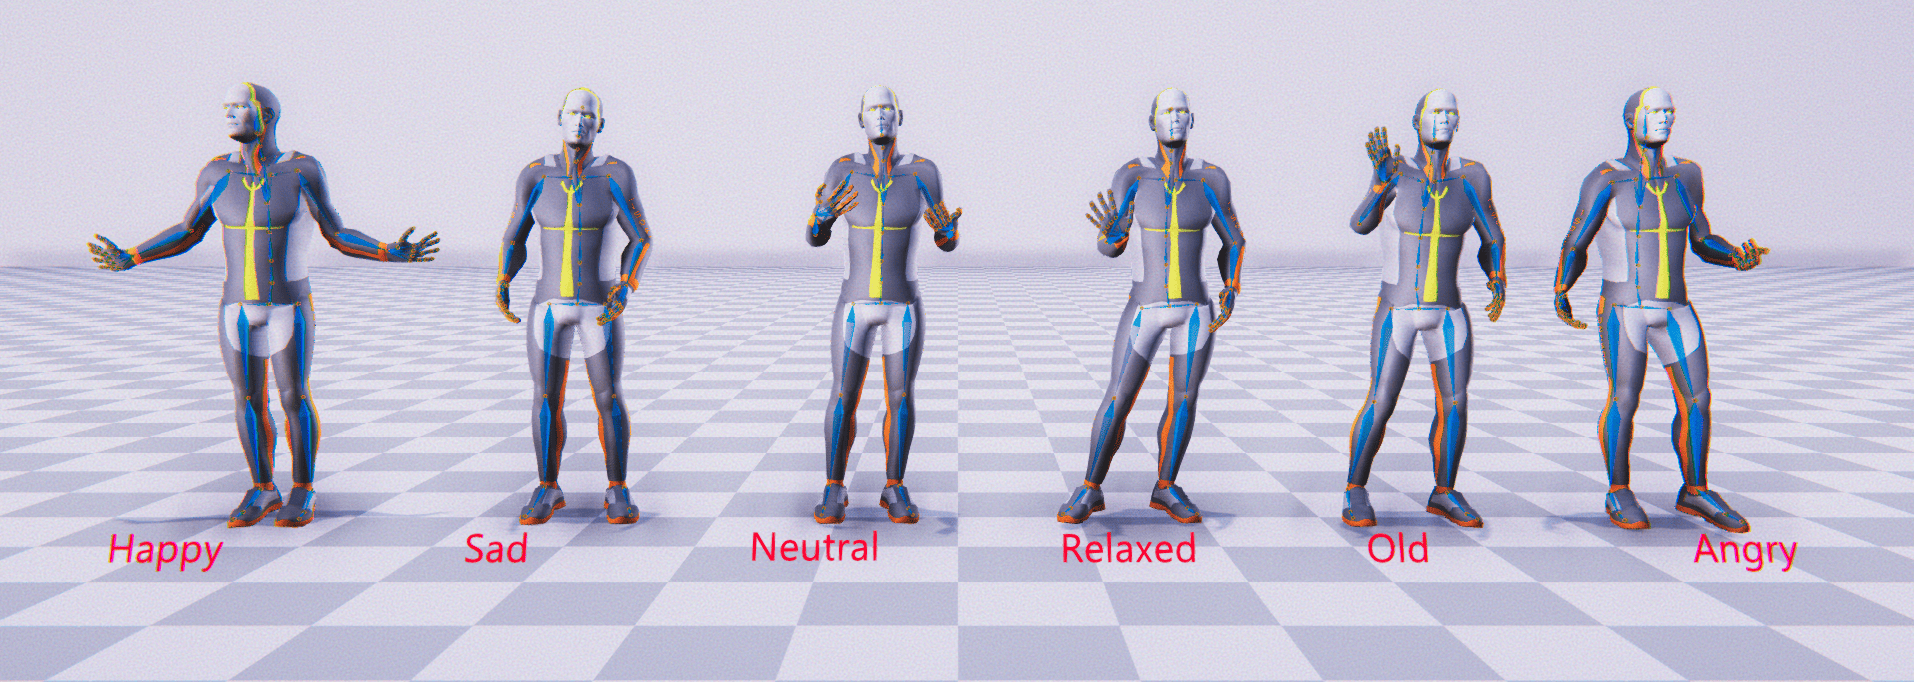
\includegraphics[width=\linewidth]{figures/EmotionAnimation}
%	\caption{Illustration of 6 gestures: $\texttt{Happy}$, $\texttt{Sad}$, $\texttt{Neutral}$, $\texttt{Old}$, $\texttt{Relaxed}$, and $\texttt{Angry}$}
%\end{figure}

\begin{figure}[htbp]
	\centering
	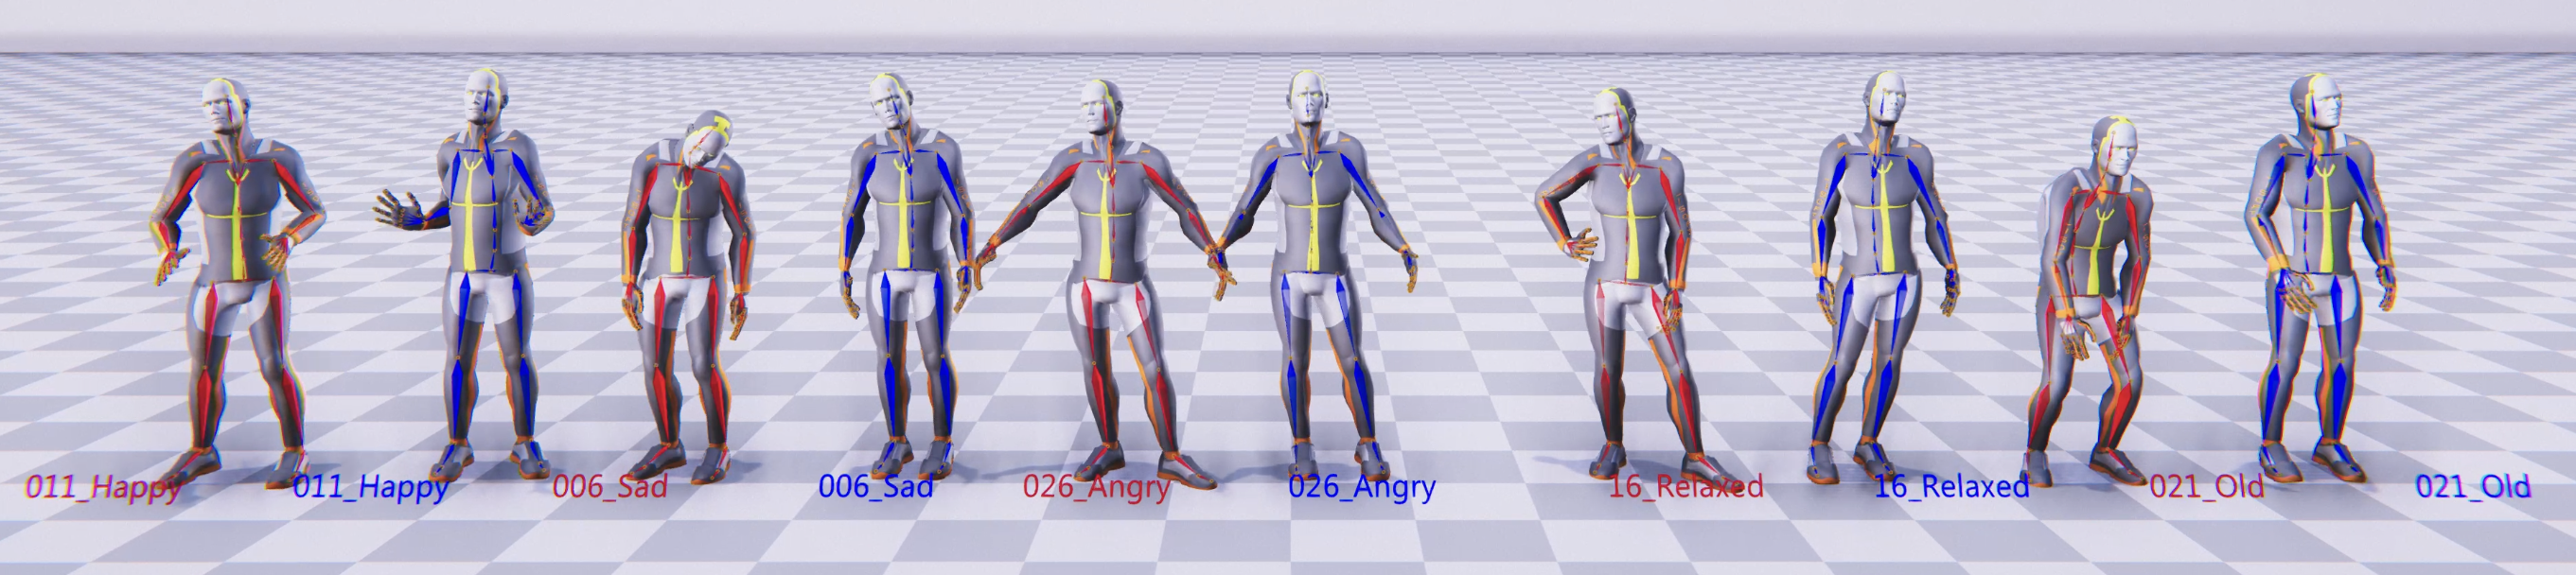
\includegraphics[width=\linewidth]{figures/DifferenceEmotion}
	\caption{Gesture samples of difference emotion}
\end{figure}

We uses the ZeroEGGS retarget dataset \cite{ghorbani2022zeroeggs}, \cite{ghorbani2022zeroeggszeroshotexamplebasedgesture}, a motion capture dataset designed for research and development of gesture generation models. It includes 67 monologue clips performed by a female motion capture actor, with a total duration of 135 minutes. The monologues are annotated with 6 different emotions: $\texttt{Happy}$, $\texttt{Sad}$, $\texttt{Neutral}$, $\texttt{Old}$, $\texttt{Relaxed}$, and $\texttt{Angry}$, enabling simulation of various emotional states in gestures and body movements. ZeroEGGS provides a rich platform for studying the integration of speech and dynamic gestures, supporting the development of models capable of adapting gestures according to emotions and text semantics.

\subsection{Data Preprocessing}
\label{sec:Preprocessing}

In stage {1. Data Preprocessing} (\autoref{fig:CommonStage}), gesture, speech, and text data are read and processed to be represented as vectors or matrices containing information derived from raw data.

For \textbf{text data}: we use the $\texttt{nltk}$ library for tokenization and $\texttt{contractions}$ to normalize contracted words.

One of our contributions is converting the speech data available in ZeroEGGS using Adobe Speech To Text, then align the phonetic timestamps using the Montreal Forced Aligner \cite{saxon2020robust} with an English phoneme dictionary to match the gesture frame rate, generating TextGrid files. From these TextGrids containing word-level timing information, we use $\texttt{gensim}$ to generate word2vec embeddings.

\textbf{Gesture data} consists of BVH (BioVision Motion Capture) files captured via motion capture systems. BVH files include two components: Hierarchy and Motion. Specifically:

\begin{itemize}
	\item \texttt{HIERARCHY}: defines a skeletal tree containing 75 bones $\{ \mathbf{b}_1, \mathbf{b}_2 \cdots \mathbf{b}_{75} \}$, each with an initial position (\texttt{OFFSET}) and \texttt{CHANNELS} parameters specifying the type and order of rotation angles (\texttt{Zrotation}, \texttt{Yrotation}, \texttt{Xrotation}) and position (\texttt{Xposition}, \texttt{Yposition}, \texttt{Zposition}), which are defined in the \texttt{MOTION} section. The first bone (usually \texttt{Hips}) is the root bone $\mathbf{b}_{\text{root}}$, used to define the T-pose via forward kinematics as the initial pose of the skeleton before applying motion.
	
	\item \texttt{MOTION}: a sequence of frames, each containing motion data representing changes of all $75$ bones as defined by the \texttt{CHANNELS} in the \texttt{HIERARCHY}.
\end{itemize}

Our model converts Euler rotation angles to quaternion rotation angles, where a quaternion is a 4-dimensional vector.

\begin{equation} \label{eq:gesturevector}
	\mathbf{g} = \Big[ \mathbf{p}_{\text{root}},  \mathbf{r}_{\text{root}},
	\mathbf{ p }'_{\text{root}},  \mathbf{r}'_{\text{root}},
	\mathbf{p}_{\text{joins}},  \mathbf{r}_{\text{joins}},
	\mathbf{p}'_{\text{joins}},  \mathbf{r}'_{\text{joins}},
	\mathbf{d}_{\text{gaze}}
	\Big]
\end{equation}

Here, each $\mathbf{g} \in \mathbb{R}^{1141}$ includes:
{
	\begin{itemize}
		\item $\mathbf{p}_{\text{root}} \in \mathbb{R}^3$: coordinates of the root joint
		\item $\mathbf{r}_{\text{root}} \in \mathbb{R}^4$: rotation (quaternion) of the root joint
		\item $\mathbf{p}'_{\text{root}} \in \mathbb{R}^3$: velocity of the root position
		\item $\mathbf{r}'_{\text{root}} \in \mathbb{R}^3$: angular velocity of the root rotation
		
		\item $\mathbf{p}_{\text{joins}} \in \mathbb{R}^{3 n_{\text{join} }}$: positions of other joints
		\item $\mathbf{r}_{\text{joins}} \in \mathbb{R}^{6 n_{\text{join} }}$: joint rotations on the X and Y planes
		\item $\mathbf{p}'_{\text{joins}} \in \mathbb{R}^{3n_{\text{join} }}$: velocity of joint positions
		\item $\mathbf{r}'_{\text{joins}} \in \mathbb{R}^{3n_{\text{join} }}$: angular velocity of joint rotations
		\item $\mathbf{d}_{\text{gaze}} \in \mathbb{R}^3$: gaze direction
\end{itemize}}

The original gesture sequences in Euler angles are converted to radians, then converted from Euler to Quaternion as detailed in \autoref{appendix:BVHQuaternion}.

\textbf{Speech data}: $\mathbf{a}_{\text{raw}} \in \mathbb{R}^{ \text{length } }$ is raw speech sampled at 16000 Hz, trimmed into segments $\mathbf{a} \in \mathbb{R}^{64000}$ corresponding to 4 seconds. The paper uses \texttt{ffmpeg-normalize} to normalize volume to a level lower than the original.

\textbf{Emotion}: Emotion data is represented using a predefined one-hot encoded vector. During sampling, the filename encodes the target emotion.

All data is stored using the $\texttt{h5}$ format.

\subsection{Training Process}

The entire model training process was conducted over approximately two weeks with the following parameters: number of training steps $T = 1000$, using an Nvidia 3090 GPU. The learning rate was set to $3 \times 10^{-5}$, batch size was $640$, and a total of $43,853$ samples were trained. At each step, $t$ is randomly sampled and input to $f_{\theta}$ to predict $\mathbf{x}_{0}$. The emotional control parameter was set to $\gamma = 0.1$. The probability of applying random masking to the emotion and initial gesture matrices was $10\%$, using a Bernoulli distribution to randomly hide/reveal these matrices.

The $\beta$ parameter was scheduled linearly from $0.5 \rightarrow 0.999$.

The $\operatorname{HuberLoss} (\mathbf{x}_{0},  \hat{\mathbf{x}}_{0} )$ is computed as follows:

\begin{itemize}
	\item If $|\mathbf{x}_0 - \hat{\mathbf{x}}_0| \leq \delta$ then $\mathcal{L}_{ \delta, \mathbf{x}_0, \hat{\mathbf{x}}_0} = \frac{1}{2} (\mathbf{x}_0 - \mathbf{x}_0)^2$: Below the threshold, the loss is computed as squared distance (similar to MSE), which is sensitive to small errors and provides smooth gradients.
	
	\item If $|\mathbf{x}_0 - \hat{\mathbf{x}}_0| > \delta$ then $\mathcal{L}_{ \delta, \mathbf{x}_0, \hat{\mathbf{x}}_0}  =  \delta \cdot |\mathbf{x}_0 - \mathbf{x}_0| - \frac{1}{2} \delta^2$: Above the threshold, the loss behaves like MAE, reducing sensitivity to large errors and improving robustness against outliers.
	
\end{itemize}

The training process is implemented in the open-source repository: \hyperlink{https://github.com/DeepGesture/DeepGesture}{Github/DeepGesture} \footnote{\url{https://github.com/DeepGesture/DeepGesture}}.

\subsection{Rendering Process in Unity}
\label{sec:Render}

To visualize the gesture generation process from model output, we use Unity in stage \textit{7. Rendering} (\autoref{fig:CommonStage}), extending code from the DeepPhase model \cite{starke2022deepphase}. The generated output is in BVH (BioVision Motion Capture) format. In Unity, the author adds C-Sharp scripts to render gestures based on coordinates and labels, with bone positions and rotations represented using quaternions.

Rendering details are presented in \autoref{appendix3}.

The Unity project source code is available at: \hyperlink{https://github.com/DeepGesture/deepgesture-unity}{Github/DeepGesture-Unity}
\footnote{\url{https://github.com/DeepGesture/deepgesture-unity}}.










%\section{Data Preparation}
%\label{sec:data_preparation}
%The \emph{data} module of our system preprocesses an input speech, segments it into uniform blocks based on speech rhythms, and extracts features that will be used to generate co-speech gestures. In this section, we first introduce the representations of different speech modalities and gesture motion and then describe details of the data preprocessing.
%
%\subsection{Representation of Speech Modalities}
%
%\subsubsection{Motion Representation}
%%
%\begin{figure}[t]
%	\centering
%	\includegraphics[width=0.9\linewidth]{figures/skeleton.pdf}
%	\caption{The character model used in our system.}
%	\label{fig:character_model}
%\end{figure}
%%
%We focus on upper-body gestures in this work. Our system employs a character model consisting of $16$ upper-body joints, including a rotational root, as shown in \fig\ref{fig:character_model}. A gesture pose is then represented as a list of joint rotations, parameterized using the exponential map, in the hierarchical order. We use $\vect{m}_k\in\mathbb{R}^{d_m}$ to represent the gesture pose at frame $k$, and a clip of gestures is  represented collectively as $\vect{M}=\{\vect{m}_1,\dots,\vect{m}_K\}$, where $K$ is the number of frames. We retarget training motions onto this model by copying the rotations of corresponding joints. The translation and the rotation around the vertical axis are excluded from the root joint, ensuring a normalized body orientation.
%
%\subsubsection{Text Representation}
%Text transcription is an important speech modality that provides high-level linguistic information in a compact format. It is typically given as a word sequence, where the number of words per unit time can vary depending on the speed of the speech. Following \cite{kucherenko2020gesticulator}, we align the words to the speech and convert the text into frame-level features to overcome this issue, which is done using an off-the-shelf text-speech alignment tool combined with a pre-trained language model.
%
%Text-speech alignment is a standard technique in the field of speech synthesis. In our system, we employ Montreal Forced Aligner (MFA) \cite{mcauliffe2017montreal} for this task, which pinpoints the beginning and end frames of every word in the speech. MFA also identifies silences and represents them as empty words. Since a speaker typically stops gesticulating in a long silence~\cite{graziano2018silence}, our system records those silences and uses them during training to reproduce such behaviors, as will be detailed later.
%
%We then pass the text and the empty words into BERT~\cite{devlin2019bert}, a popular and powerful pre-trained language model, to extract a high-level representation of the text. BERT computes an encoding vector for each word in an input sentence, which is then repeated and used for all the frames that the word occupies. We represent these word vectors collectively as $\vect{T}=\{\vect{t}_1,\dots,\vect{t}_K\}$ for a speech clip of $K$ frames, where each $\vect{t}\in\mathbb{R}^{d_t}$.
%
%\subsubsection{Audio Representation}
%\label{subsubsec:audio_representation}
%%
%\begin{figure}[t]
%	\centering
%	\includegraphics[width=\linewidth]{figures/fig2a.pdf}
%	\caption{A contrastive learning task is performed to disentangle multi-level audio features. We use the text feature $\vect{t}$ as the anchor of this learning. The highest-level audio feature $\vect{a}^{\eqword{high}}$ is considered as the positive sample, while the features of the lower levels are all treated as negative samples. After training, both $\vect{a}^{\eqword{high}}$ and the feature extracted at the second level, $\vect{a}^{\eqword{low}}$, are used for gesture generation.}
%	\label{fig:audio_feature_extraction}
%\end{figure}
%%
%Many recent studies use deep encoders to extract audio features from raw audio signals or audio spectrograms, where only the features extracted at the last layer of the encoder are used to generate gestures~\cite{yoon2020speech,alexanderson2020style,kucherenko2020gesticulator,qian2021speech,li2021audio2gestures}. Such a configuration potentially encourages the encoder to mix information from multiple levels into the same feature, which can be difficult to disentangle in the downstream generation tasks.
%
%In our system, we propose to decouple the multi-level audio features in the encoder and use them in different scenarios. We assume the high-level features correspond to the speech semantics that determines the gesture lexemes, while the low-level features relate to the other audio information and can be used to control the {gesture styles}. As shown in \fig\ref{fig:audio_feature_extraction}, we employ a pre-trained speech model, {vq-wav2vec}~\cite{baevski2020vq-wav2vec}, to extract audio features from raw audio signals and fine-tune it using a contrastive learning strategy.
%
%The encoder of vq-wav2vec has $L=8$ convolutional layers. When taking a block of audio signals of $K$ frames, $\vect{A}$, as input, this encoder produces a representation $\vect{a}_k$ for each frame $k$ of the audio. In this computation, the outputs of every layer can be considered as a set of multi-level features $\{\vect{a}_k^{l}\}, {l=1,\dots,L}$, and notably, $\vect{a}_k^{L}=\vect{a}_k$. We then encourage the highest-level feature $\vect{a}_k^{L}$ to match the speech content and push apart the features of the lower levels $\{\vect{a}_k^{l}\}, l<L$ to capture crucial content-irrelevant information. Specifically, we utilize the contrastive loss
%\begin{equation}
%	\mathcal{L}_{\eqword{cont}} = -\log{\frac{\exp{(\simloss(\tildevect{t}_{k}, \tildevect{a}^{L}_{k})/\tau)}}{\sum^{K}_{i=1}\sum_{l=1}^{L}\exp{(\simloss(\tildevect{t}_k, \tildevect{a}^{l}_{i})}/\tau)}},
%\end{equation}
%where the text feature $\vect{t}_k$ is extracted from the speech transcription, the $\simloss(\cdot,\cdot)$ function computes the cosine similarity between two vectors as
%\begin{equation}
%	\simloss(\tildevect{t},\tildevect{a})=\frac{\tildevect{t} \cdot \tildevect{a}}{\norm{\tildevect{t}}\norm{\tildevect{a}}},
%\end{equation}
%and $\tau$ is the temperature hyperparameter. All the feature vectors are projected into the same vector space using learnable linear projections $\tildevect{t}=F_t(\vect{t})$ and $\tildevect{a}_k^l=F_a^l(\vect{a}_k^l)$, $l=1,\dots,L$, respectively. Notably, we consider the highest-level audio feature of the current frame as the positive example and audio features of the other levels and the other frames as the negative examples in this contrastive learning process.
%
%This contrastive learning strategy is partially inspired by the HA2G model proposed by Liu et al.~\shortcite{liu2022learning}. However, unlike their approach, which considers contrastive learning as a part of the training of the gesture generator, we train the audio encoder in a separate pre-training stage using only the speech data. After the training, the features extracted at the second and the last layers of the encoder, represented by $\vect{a}^{\eqword{low}}\in\mathbb{R}^{d_a}$ and $\vect{a}^{\eqword{high}}\in\mathbb{R}^{d_A}$, respectively, are then used in different training and inference stages in the downstream generation task. They can be represented collectively as $\vect{A}^{\eqword{low}}$ and $\vect{A}^{\eqword{high}}$ for a speech clip. Although the gesture motions are not considered here, we find that the results of this encoder still demonstrate correlations between the high-level audio features and the gestures. We will discuss these results later in Section~\ref{subsec:ablation_study}.
%
%\subsubsection{Identity Representation}
%Similar to previous studies \cite{yoon2020speech,bhattacharya2021speech2affectivegestures}, our system can leverage the speaker identity (ID) to help distinguish different gesture styles and achieve stylized gesture generation. We represent each speaker as a one-hot vector $\vect{I}\in\{0,1\}^{N_I}$, where $N_I$ is the number of speakers in a dataset.
%%
%\begin{figure}[t]
%	\centering    
%	\begin{subfigure}[t]{0.47\linewidth}
%		\centering
%		\caption*{Trinity Gesture Dataset}
%		\includegraphics[width=\linewidth]{figures/onset_interval_trinity.pdf}
%	\end{subfigure}
%	\hspace{\fill}
%	\begin{subfigure}[t]{0.47\linewidth}
%		\centering
%		\caption*{TED Gesture Dataset}
%		\includegraphics[width=\linewidth]{figures/onset_interval_TED.pdf}
%	\end{subfigure}
%	\caption{Distribution of time intervals between consecutive audio onsets in two open-source speech-gesture datasets.}
%	\label{fig:onset_intervals}
%\end{figure}
%%
%\subsection{Rhythm-Based Speech Segmentation}
%\label{subsec:beat_alignment}
%In this section, we describe how our system segments and normalizes an input speech into uniform blocks. This procedure is crucial for generating a gesture motion that is temporally synchronized with the rhythm of the speech. To that end, our system first identifies beats in the input audio, which generally corresponds to phonetic properties such as stress or accent, then segments the speech at every beat and time-scales the audio to the same length.
%
%\subsubsection{Beat Identification}
%\label{subsubsec:onset_identification}
%Rhythm can be characterized by a pattern of beats. In music-related tasks, such as dance generation~\cite{chen2021choreomaster,aristidou2021rhythm}, identifying beats using the onsets of audio signals is a standard technique~\cite{bello2005onsetTutorial,ellis2007beat}, where off-the-shelf tools such as librosa library~\cite{mcfee2015librosa} can be employed to extract those audio features.
%
%However, unlike the rhythm in music that is typically consistent over time, the pattern of beats in a speech can vary significantly according to the context and pace of the speech. Taking a close look at the time intervals between consecutive audio onsets in our training dataset, we notice that the majority of those intervals fall within a range roughly between $D_m=0.2\sim{}0.3$ seconds and $D_M=0.5\sim{}0.6$ seconds, as illustrated in \fig\ref{fig:onset_intervals}, though the actual values of $D_m$ and $D_M$ may vary among datasets depending on the personality of the speakers and the language they speak. We also observe that the time intervals shorter than $D_m$ are often caused by noise, filler words, or stuttering. On the other hand, the intervals that are excessively long often correspond to pauses or silent periods.
%
%Based on these observations, our system employs a simple heuristic strategy to identify beats based on the audio onsets. An onset will be recognized as a beat unless the time interval between it and the previous beat is shorter than $D_m$, in which case the onset will be ignored. If an interval is longer than $D_M$, we will insert a necessary number of \emph{pseudo-beat}s to make the duration of every new interval within the range $[D_m, D_M]$. More specifically, we insert a pseudo-beat at the first frame which is $D_m$ seconds away from any preceding beat and where the volume of the audio is greater than a threshold $\tilde{I}_a$. Other pseudo-beats are then added recursively in the same way. We set the threshold $\tilde{I}_a$ as the average volume of the environmental noise. If the entire interval is quieter than $\tilde{I}_a$, a minimal number of pseudo-beats will be placed evenly in it so that each new interval is shorter than $D_M$.
%
%\subsubsection{Normalization}
%\label{subsubsec:normalization}
%Our system then segments the speech into short clips at every beat. These clips are then time-scaled into uniform blocks of length $D_M$. The speech modalities are segmented and time-scaled as well in this process. For the motion, $\vect{M}$, and text representation, $\vect{T}$, of a clip, we resample the corresponding features to match the new length. The audio is processed with additional care, where we use the TSM (Time-Scale Modification) algorithm to change the duration of the audio while preserving the pitch. The audio features $\vect{A}^{\eqword{low}}$ and $\vect{A}^{\eqword{high}}$ are then recomputed for the time-scaled audio blocks. The speaker ID $\vect{I}$ is a constant of the whole speech, which will not be changed during the normalization.